\section{Cài đặt và thử nghiệm}

\subsection{Môi trường thử nghiệm}
\begin{frame}{\secname: \subsecname}

    Thử nghiệm được thực hiện trên nền tảng Kaggle với cấu hình GPU T4 x2.

    \bigskip
    Mô hình được huấn luyện riêng biệt trên hai tập dữ liệu QaTa-COV19-v2 và MosMedData+. Hai tập dữ liệu này đều có mặt nạ phân đoạn và ghi chú y khoa đi kèm, do đó phù hợp với mục tiêu đánh giá mô hình phân đoạn đa phương thức dựa trên cả thông tin ảnh và văn bản.

    \bigskip
    Trước khi đưa vào mô hình, tất cả ảnh đầu vào được thay đổi kích thước về $224 \times 224$. Đây là kích thước đầu vào phổ biến của Vision Transformer, đặc biệt trong các mô hình tiền huấn luyện trên ImageNet.
\end{frame}

\begin{frame}{\secname: \subsecname}

    \begin{table}[H]
        \centering
        \begin{tabular}{lcccc}
        \hline
        \multirow{2}{*}{} & \multicolumn{2}{c}{\textbf{QaTa-COV19-v2}} & \multicolumn{2}{c}{\textbf{MosMedData+}} \\
        \cline{2-5}
        & Supervised & Semi-supervised & Supervised & Semi-supervised \\
        \hline
        \textbf{Optimizer} & \multicolumn{4}{c}{Adam} \\
        \textbf{Tỉ lệ nhãn} & 100\% & 25\% & 100\% & 25\% \\
        \textbf{Batch size} & 24 & 16 & 24 & 16 \\
        \textbf{LR} & \multicolumn{2}{c}{0.0003} & \multicolumn{2}{c}{0.001} \\
        \textbf{Scheduler} & \multicolumn{4}{c}{Cosine Annealing Restarts} \\
        \textbf{Epochs} & \multicolumn{4}{c}{100} \\
        \hline
        \end{tabular}
    \end{table}
\end{frame}

\subsection{Cài đặt thực tế}

\begin{frame}{\secname: \subsecname}

    \begin{figure}[H]
        \centering
        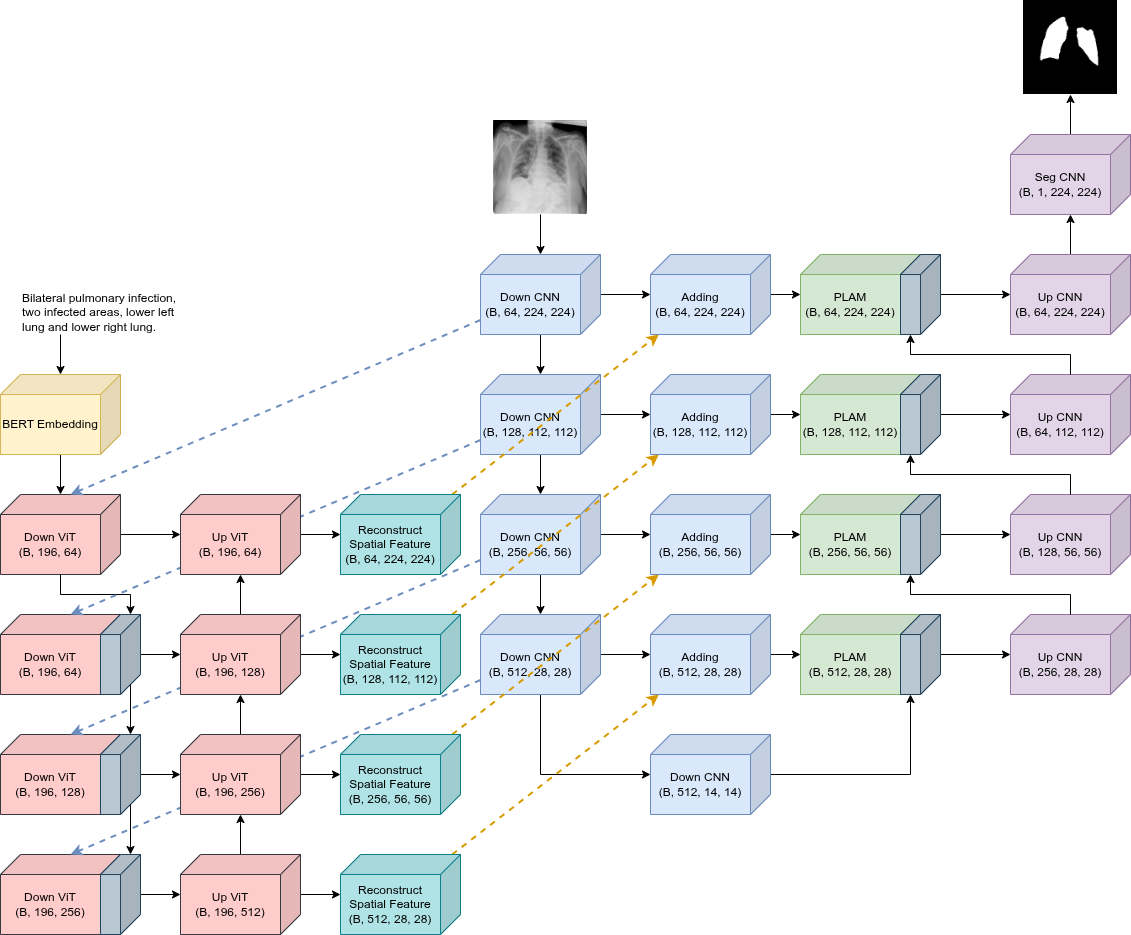
\includegraphics[width=0.7\linewidth]{images/implementation.png}
        \caption{Minh họa kiến trúc LViT trong cài đặt.}
    \end{figure}

\end{frame}

\begin{frame}{\secname: \subsecname}

    \begin{figure}[H]
        \centering
        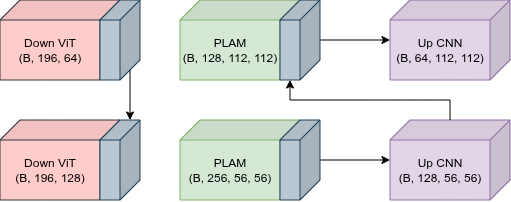
\includegraphics[width=0.7\linewidth]{images/concat.png}
        \caption{Phép nối dữ liệu theo chiều kênh.}
    \end{figure}
\end{frame}

\subsection{Kết quả thử nghiệm}
\begin{frame}{\secname: \subsecname}

    \begin{figure}[H]
        \centering
        \setlength{\tabcolsep}{2pt}
        \begin{tabular}{cccccccc}
            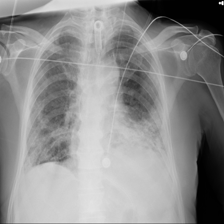
\includegraphics[width=0.115\linewidth]{comparison/sub-S08047_ses-E16280_run-1_bp-chest_vp-ap_dx.png} &
            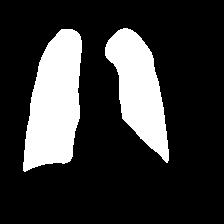
\includegraphics[width=0.115\linewidth]{comparison/sub-S08047_ses-E16280_run-1_bp-chest_vp-ap_dx.png_lab.jpg} &
            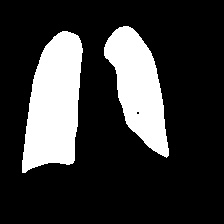
\includegraphics[width=0.115\linewidth]{comparison/sub-S08047_ses-E16280_run-1_bp-chest_vp-ap_dx.png_predictSupervisedLViT.jpg} &
            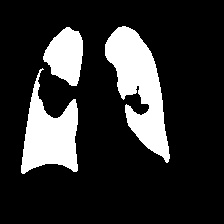
\includegraphics[width=0.115\linewidth]{comparison/sub-S08047_ses-E16280_run-1_bp-chest_vp-ap_dx.png_predictSemiLViT.jpg} &
            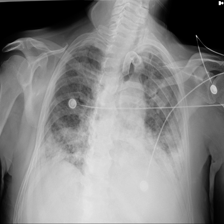
\includegraphics[width=0.115\linewidth]{comparison/sub-S08047_ses-E16628_run-1_bp-chest_vp-ap_dx.png} &
            
\includegraphics[width=0.115\linewidth]{comparison/sub-S08047_ses-E16628_run-1_bp-chest_vp-ap_dx.png_lab.jpg} &
            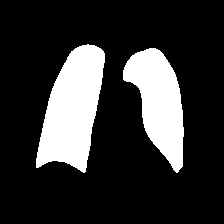
\includegraphics[width=0.115\linewidth]{comparison/sub-S08047_ses-E16628_run-1_bp-chest_vp-ap_dx.png_predictSupervisedLViT.jpg} &
            
\includegraphics[width=0.115\linewidth]{comparison/sub-S08047_ses-E16628_run-1_bp-chest_vp-ap_dx.png_predictSemiLViT.jpg} \\
            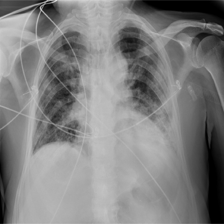
\includegraphics[width=0.115\linewidth]{comparison/sub-S08047_ses-E16837_run-1_bp-chest_cr.png} &
            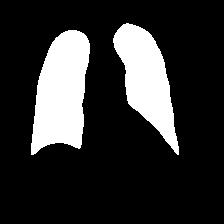
\includegraphics[width=0.115\linewidth]{comparison/sub-S08047_ses-E16837_run-1_bp-chest_cr.png_lab.jpg} &
            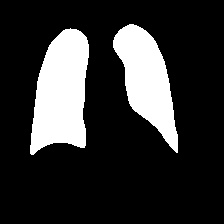
\includegraphics[width=0.115\linewidth]{comparison/sub-S08047_ses-E16837_run-1_bp-chest_cr.png_predictSupervisedLViT.jpg} &
            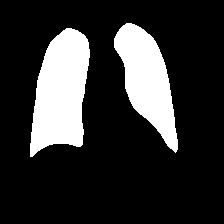
\includegraphics[width=0.115\linewidth]{comparison/sub-S08047_ses-E16837_run-1_bp-chest_cr.png_predictSemiLViT.jpg} &
            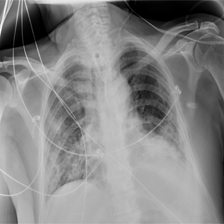
\includegraphics[width=0.115\linewidth]{comparison/sub-S08047_ses-E17130_run-1_bp-chest_cr.png} &
            
\includegraphics[width=0.115\linewidth]{comparison/sub-S08047_ses-E17130_run-1_bp-chest_cr.png_lab.jpg} &
            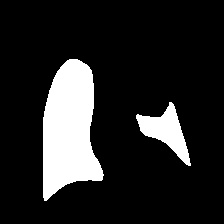
\includegraphics[width=0.115\linewidth]{comparison/sub-S08047_ses-E17130_run-1_bp-chest_cr.png_predictSupervisedLViT.jpg} &
            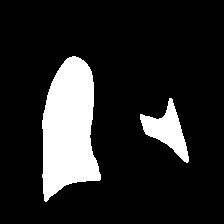
\includegraphics[width=0.115\linewidth]{comparison/sub-S08047_ses-E17130_run-1_bp-chest_cr.png_predictSemiLViT.jpg} \\
        \end{tabular}
        \caption{So sánh trực quan dự đoán trên QaTa-COV19, thứ tự từ trái sang phải là ảnh gốc, ground truth, mask supervised và mask semi-supervised.}
    \end{figure}

\end{frame}

\begin{frame}{\secname: \subsecname}

    \begin{figure}[H]
        \centering
        \setlength{\tabcolsep}{2pt}
        \begin{tabular}{cccccccc}
            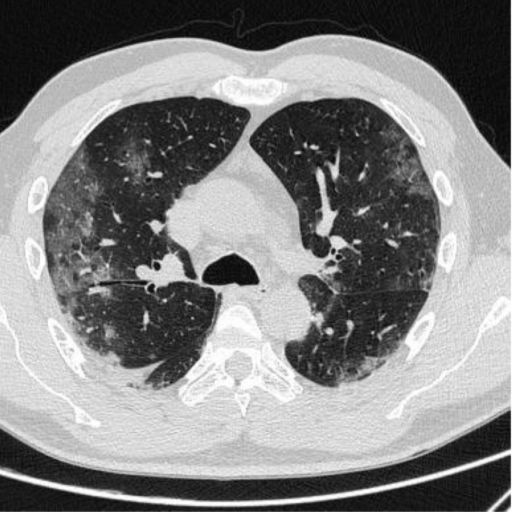
\includegraphics[width=0.115\linewidth]{comparison2/bjorke_81.png} &
            
\includegraphics[width=0.115\linewidth]{comparison2/bjorke_81.png_lab.jpg} &
            
\includegraphics[width=0.115\linewidth]{comparison2/bjorke_81.png_predictSupervisedLViT.jpg} &
            
\includegraphics[width=0.115\linewidth]{comparison2/bjorke_81.png_predictSemiLViT.jpg} &
            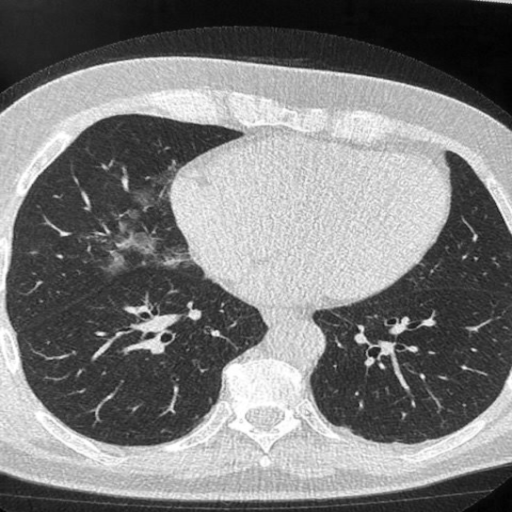
\includegraphics[width=0.115\linewidth]{comparison2/bjorke_82.png} &
            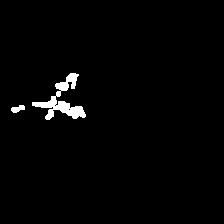
\includegraphics[width=0.115\linewidth]{comparison2/bjorke_82.png_lab.jpg} &
            
\includegraphics[width=0.115\linewidth]{comparison2/bjorke_82.png_predictSupervisedLViT.jpg} &
            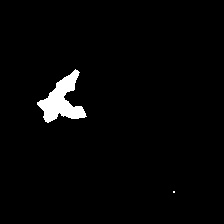
\includegraphics[width=0.115\linewidth]{comparison2/bjorke_82.png_predictSemiLViT.jpg} \\
            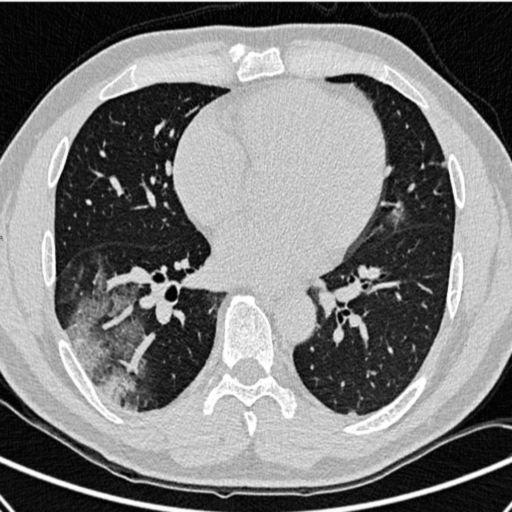
\includegraphics[width=0.115\linewidth]{comparison2/bjorke_83.png} &
            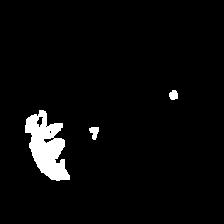
\includegraphics[width=0.115\linewidth]{comparison2/bjorke_83.png_lab.jpg} &
            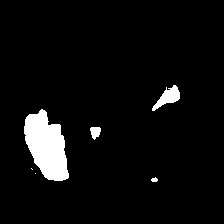
\includegraphics[width=0.115\linewidth]{comparison2/bjorke_83.png_predictSupervisedLViT.jpg} &
            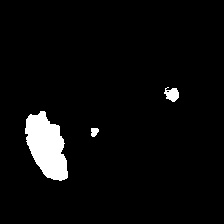
\includegraphics[width=0.115\linewidth]{comparison2/bjorke_83.png_predictSemiLViT.jpg} &
            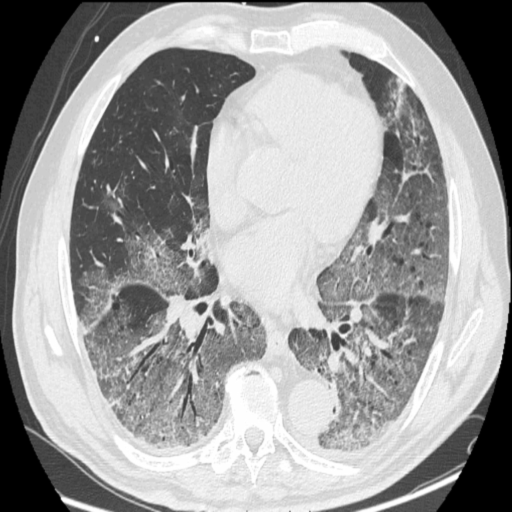
\includegraphics[width=0.115\linewidth]{comparison2/bjorke_9.png} &
            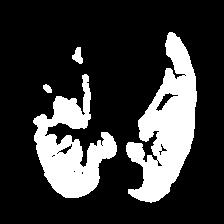
\includegraphics[width=0.115\linewidth]{comparison2/bjorke_9.png_lab.jpg} &
            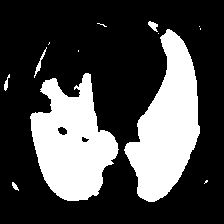
\includegraphics[width=0.115\linewidth]{comparison2/bjorke_9.png_predictSupervisedLViT.jpg} &
            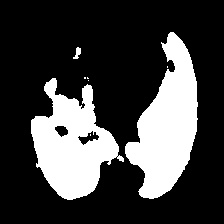
\includegraphics[width=0.115\linewidth]{comparison2/bjorke_9.png_predictSemiLViT.jpg} \\
        \end{tabular}
        \caption{So sánh trực quan dự đoán trên MosMedData+, thứ tự trong mỗi nhóm là ảnh gốc, ground truth, mask supervised và mask semi-supervised.}
    \end{figure}

\end{frame}

\begin{frame}{\secname: \subsecname}

    \begin{table}[H]
        \centering
        \caption{Kết quả huấn luyện, kiểm định và kiểm thử của LViT trên các cấu hình thực nghiệm}
        \resizebox{\linewidth}{!}{%
            \begin{tabular}{lccccc}
            \hline
            \textbf{Dữ liệu} & \textbf{Cấu hình} & \textbf{Train Dice} & \textbf{Val Dice} & \textbf{Test Dice} & \textbf{Test IoU} \\
            \hline
            Covid19 & Supervised & 86.32 & 79.44 & 81.27 & 72.46 \\
            Covid19 & Semi-supervised & 85.91 & 75.28 & 76.72 & 66.93 \\
            MosMedData+ & Supervised & 79.73 & 67.20 & 13.39 & 11.00 \\
            MosMedData+ & Semi-supervised & 78.79 & 63.86 & 12.92 & 10.44 \\
            \hline
            \end{tabular}%
        }
    \end{table}

\end{frame}


\begin{frame}{\secname: \subsecname}

    Trên tập Covid19, mô hình đạt kết quả tương đối ổn định, cho thấy khoảng cách giữa huấn luyện, kiểm định và kiểm thử không quá lớn. Khi chuyển sang cấu hình semi-supervised, Test Dice và Test IoU đều giảm. Mức giảm này là hợp lý vì mô hình không còn được sử dụng đầy đủ nhãn thật trong quá trình huấn luyện, trong khi phần sinh nhãn giả trong mã nguồn tái lập không hoàn toàn tương đương với một quy trình bán giám sát hoàn chỉnh trong công trình gốc.

    \bigskip
    Trên tập MosMedData+, kết quả có sự khác biệt rõ rệt giữa train/validation và test. Cả supervised và semi-supervised đều có sự giảm mạnh. Điều này cho thấy mô hình có học được đặc trưng trên tập huấn luyện, nhưng khả năng tổng quát hóa sang tập kiểm thử của MosMedData+ chưa tốt.

\end{frame}

\begin{frame}{\secname: \subsecname}

   Nguyên nhân kết quả trên MosMedData+ thấp có thể đến từ ba yếu tố chính:

   \begin{itemize}
       \item MosMedData+ là dữ liệu CT, khác biệt rõ với ảnh X-ray của Covid19 về cấu trúc lát cắt, độ tương phản và phân bố cường độ.
       \item Dữ liệu tái lập có thể khác công trình gốc về cách tổ chức, định dạng, ánh xạ mặt nạ và chia tập dữ liệu.
       \item Thời gian huấn luyện trên Kaggle bị giới hạn, mô hình dùng số epoch cố định nên có thể chưa hội tụ tốt trên MosMedData+.
   \end{itemize}

\end{frame}

\begin{frame}{\secname: \subsecname}

    \begin{table}[H]
        \centering
        \caption{Kết quả so sánh LViT thử nghiệm với LViT công bố và các phương pháp SOTA}
        \resizebox{\linewidth}{!}{%
        \begin{tabular}{lcccccc}
        \hline
        \multirow{2}{*}{\textbf{Phương pháp}} & \multirow{2}{*}{\textbf{Văn bản}} & \multirow{2}{*}{\textbf{Tỉ lệ nhãn}} & \multicolumn{2}{c}{\textbf{QaTa-COV19}} & \multicolumn{2}{c}{\textbf{MosMedData+}} \\
        \cline{4-7}
        & & & Dice (\%) & mIoU (\%) & Dice (\%) & mIoU (\%) \\
        \hline
        \textbf{LViT-T-Exp} (1/4) & $\checkmark$ & 25\% & 76.72 & 66.93 & 12.92 & 10.44 \\
        \textbf{LViT-T-Exp} & $\checkmark$ & 100\% & 81.27 & 72.46 & 13.39 & 11.00 \\
        \hline
        LViT-TW (1/4) & $\times$ & 25\% & 79.08 & 69.42 & 70.65 & 58.07 \\
        LViT-TW (1/2) & $\times$ & 50\% & 80.35 & 70.74 & 71.89 & 59.63 \\
        LViT-TW & $\times$ & 100\% & 81.12 & 71.37 & 72.58 & 60.40 \\
        LViT-T (1/4) & $\checkmark$ & 25\% & 80.95 & 71.31 & 72.48 & 60.31 \\
        LViT-T (1/2) & $\checkmark$ & 50\% & 82.73 & 73.99 & 73.56 & 61.05 \\
        LViT-T & $\checkmark$ & 100\% & 83.66 & 75.11 & 74.57 & 61.33 \\
        \hline
        U-Net & $\times$ & 100\% & 79.02 & 69.46 & 64.60 & 50.73 \\
        UNet++ & $\times$ & 100\% & 79.62 & 70.25 & 71.75 & 58.39 \\
        nnUNet & $\times$ & 100\% & 80.42 & 70.81 & 72.59 & 60.36 \\
        \hline
        GLoRIA & $\times$ & 100\% & 79.94 & 70.68 & 72.42 & 60.18 \\
        LAVT & $\times$ & 100\% & 79.28 & 69.89 & 73.29 & 60.41 \\
        \hline
        \end{tabular}%
        }
    \end{table}

\end{frame}


\begin{frame}{\secname: \subsecname}

\textbf{Phân tích trên Covid19}

\begin{itemize}
    \item Với 100\% nhãn, mô hình tái lập đạt 81.27\% Dice và 72.46\% mIoU, chỉ thấp hơn LViT-T công bố 2.39 điểm Dice.
    \item Khoảng cách này tương đối nhỏ, cho thấy pipeline tái lập trên Covid19 vẫn giữ được phần lớn hiệu quả của LViT.
    \item Với 25\% nhãn, kết quả giảm mạnh hơn, cho thấy thiết lập bán giám sát chưa tái hiện đầy đủ cơ chế của công trình gốc.
\end{itemize}

\end{frame}

\begin{frame}{\secname: \subsecname}

\textbf{Phân tích trên MosMedData+}

\begin{itemize}
    \item Kết quả tái lập trên MosMedData+ thấp hơn rất nhiều so với kết quả công bố ở cả 100\% và 25\% nhãn.
    \item Train Dice và Val Dice vẫn khá cao, nhưng Test Dice thấp, cho thấy mô hình chưa tổng quát tốt sang tập kiểm thử.
    \item Nguyên nhân có thể liên quan đến khác biệt dữ liệu CT, tiền xử lý, cách chia tập và giới hạn thời gian huấn luyện.
\end{itemize}

\end{frame}

\begin{frame}{\secname: \subsecname}

\textbf{Vai trò của thông tin văn bản}

\begin{itemize}
    \item Trong kết quả công bố, LViT-T có dùng văn bản đều tốt hơn LViT-TW chỉ dùng ảnh.
    \item Với 100\% nhãn, Dice tăng từ 81.12\% lên 83.66\% trên QaTa-COV19.
    \item Trên MosMedData+, Dice tăng từ 72.58\% lên 74.57\%, cho thấy văn bản giúp định hướng vùng cần phân đoạn.
\end{itemize}

\end{frame}

\begin{frame}{\secname: \subsecname}

\textbf{Nhận xét về bán giám sát}

\begin{itemize}
    \item Kết quả công bố cho thấy 25\% nhãn vẫn đạt hiệu quả ổn định nhờ cơ chế sinh nhãn giả EPI.
    \item Trong tái lập, hiệu quả 25\% nhãn phụ thuộc mạnh vào mức độ hoàn chỉnh của quy trình bán giám sát.
    \item EPI có tiềm năng giảm chi phí chú thích y khoa, nhưng cần bước sinh, lọc và cập nhật nhãn giả chặt chẽ hơn.
\end{itemize}

\end{frame}